% Created 2023-11-30 Thu 21:41
% Intended LaTeX compiler: pdflatex
\documentclass[presentation, smaller]{beamer}
\usepackage[utf8]{inputenc}
\usepackage[T1]{fontenc}
\usepackage{graphicx}
\usepackage{longtable}
\usepackage{wrapfig}
\usepackage{rotating}
\usepackage[normalem]{ulem}
\usepackage{amsmath}
\usepackage{amssymb}
\usepackage{capt-of}
\usepackage{hyperref}
\usepackage{amsmath,amssymb}
\usetheme[]{default}
\usepackage{tikz}
\usetikzlibrary[topaths] \newcount\mycount
\usepackage{pgf}

\pgfmathsetseed{\number\pdfrandomseed} % to ensure that it is randomized
% use \randomseed for xelatex

\newcommand{\thecmd}[1]{%
\pgfmathsetmacro{\thenum}{int(random(ceil(#1-#1/4),floor(#1+#1/4)))}%
\thenum%
}%
\usepackage{xcolor}
\usepackage{framed}
\usepackage{amsthm}
\usepackage[utf8]{inputenc}

\colorlet{shadecolor}{CoalGray!15}

\newcommand{\propnumber}{} % initialize
\newtheorem*{prop}{Proposition \propnumber}
\newenvironment{propc}[1]
{\renewcommand{\propnumber}{#1}%
\begin{prop}}
{\end{prop}}
\frenchspacing
\usetheme{purduegold}
\author{John Biechele-Speziale, Kushagra Kapoor, Jae Heo}
\date{\today}
\title{POMDPs: Myths, Legends, and Reality}
\hypersetup{
 pdfauthor={John Biechele-Speziale, Kushagra Kapoor, Jae Heo},
 pdftitle={POMDPs: Myths, Legends, and Reality},
 pdfkeywords={},
 pdfsubject={},
 pdfcreator={Emacs 28.1 (Org mode 9.6.1)}, 
 pdflang={English}}
\begin{document}

\maketitle
\begin{frame}{Outline}
\setcounter{tocdepth}{1}
\tableofcontents
\end{frame}

\setbeamertemplate{footline}[frame number]

\section{What are POMDPs?}
\label{sec:org3c744cc}

\begin{frame}[label={sec:org25d4a61}]{POMDPs are MDPs with sensors instead of direct observation of the current state.}
\begin{itemize}
\item The sensors are some probability distribution of some observation given a certain state.
\pause
\item Unlike traditional MDPs that map from states to actions, these map from belief states(observations) to actions.
\pause
\item Exact optimal solutions yield the optimal action for each possible belief state that minimizes our cost.
\end{itemize}
\pause
\begin{center}
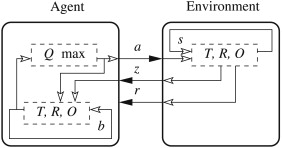
\includegraphics[width=0.8\textwidth]{fig1.jpg}
\end{center}
\end{frame}

\begin{frame}[label={sec:orgacaa6fe}]{POMDPs are defined by a tuple \((S,A,T,R,\Omega,O,\gamma)\)}
\begin{itemize}
\item S is the set of states
\pause
\item A is the set of actions
\pause
\item T is the state transition probability \(P(s'|s,a)\)
\pause
\item R is the reward function \(R(s,a)\)
\pause
\item \(\Omega\) is the set of observations
\pause
\item O is the set of conditional observation probabilities \(P(o|s') \lor P(o|s',a)\)
\pause
\item \(\gamma\) is the discount factor.
\pause
\item As usual, we want an optimal policy (\(\pi\)) that maximizes expected future reward.
\end{itemize}
\end{frame}

\begin{frame}[label={sec:orgce381a3}]{POMDPs rely on a unique belief update step as a part of the algorithm.}
\begin{itemize}
\item a
\end{itemize}
\end{frame}

\begin{frame}[label={sec:orga4e21a8}]{Notes on theory, undecidability, and intractability}
\begin{itemize}
\item 
\end{itemize}
\end{frame}

\section{POMDP Variants and Applications}
\label{sec:org7111265}

\begin{frame}[label={sec:orgd98e428}]{Various methods of solving/approximating POMDPs are currently available/used.}
\begin{itemize}
\item On Policy Methods
\begin{itemize}
\item 
\end{itemize}
\item Off Policy Methods
\begin{itemize}
\item 
\end{itemize}
\end{itemize}
\end{frame}

\section{Implementation Recommendations}
\label{sec:orgdc5a2b6}

\begin{frame}[label={sec:org763fe5c},fragile]{My favorite package: POMDPs.jl is my favorite because it's easy to use: Installation}
 \begin{verbatim}
using Pkg; Pkg.add("POMDPs"); Pkg.add("QMDP");
using POMDPs, QuickPOMDPs, POMDPTools, QMDP
\end{verbatim}
\end{frame}

\begin{frame}[label={sec:org54ffe6b},fragile]{My favorite package: POMDPs.jl is my favorite because it's easy to use: Definitions}
 \begin{verbatim}
m = QuickPOMDP(
    states = ["left", "right"],
    actions = ["left", "right", "listen"],
    observations = ["left", "right"],
    initialstate = Uniform(["left", "right"]),
    discount = 0.95,
    transition = function (s, a)
        if a == "listen"
            return Deterministic(s) # tiger stays behind the same door
        else # a door is opened
            return Uniform(["left", "right"]) # reset
        end
    end,
    observation = function (s, a, sp)
        if a == "listen"
            if sp == "left"
                return SparseCat(["left", "right"], [0.85, 0.15]) # sparse categorical distribution
            else
                return SparseCat(["right", "left"], [0.85, 0.15])
            end
        else
            return Uniform(["left", "right"])
        end
    end,
    reward = function (s, a)
        if a == "listen"
            return -1.0
        elseif s == a # the tiger was found
            return -100.0
        else # the tiger was escaped
            return 10.0
        end
    end
)

solver = QMDPSolver()
policy = solve(solver, m)

rsum = 0.0
for (s,b,a,o,r) in stepthrough(m, policy, "s,b,a,o,r", max_steps=10)
    println("s: $s, b: $([s=>pdf(b,s) for s in states(m)]), a: $a, o: $o")
    global rsum += r
end
println("Undiscounted reward was $rsum.")
\end{verbatim}

\begin{itemize}
\item \href{https://github.com/JuliaPOMDP/POMDPGallery.jl}{More Examples}
\end{itemize}
\end{frame}

\begin{frame}[label={sec:org320694b}]{Alternative Packages}
\begin{itemize}
\item \href{https://www.cs.kent.ac.uk/people/staff/mg483/code/IsoFreeBB/}{Finite-state Controllers using Branch and Bound}
\item \href{https://github.com/mhahsler/pomdp}{pomdp}
\item \href{https://bitbucket.org/bami/pypomdp}{pyPOMDP}
\item \href{https://longhorizon.org/trey/zmdp/}{zmdp}
\end{itemize}
\end{frame}
\begin{frame}[label={sec:orgdfea054}]{Temp 1}
\end{frame}

\begin{frame}[label={sec:orgf21baeb}]{Temp 2}
\end{frame}

\begin{frame}[label={sec:orgbe691ef}]{Temp 3}
\end{frame}

\begin{frame}[label={sec:orge61e3d2}]{Temp 4}
\end{frame}

\begin{frame}[label={sec:orgd687c7b}]{Temp 5}
\end{frame}

\begin{frame}[allowframebreaks,label=]{References}
\scriptsize
\bibliographystyle{plain}
\bibliography{ref}
\end{frame}
\end{document}